\label{chap:apendice}

\section{Recuperaci\'on de Informaci\'on mediante Superpixels}
\label{sec:superpixels}

La captura o recuperaci\'on de la informaci\'on del vecindario de los p\'ixeles del esqueleto se realiza utilizando la misma imagen a partir de la cual se obtiene el esqueleto, en conjunto con el grafo derivado del esqueleto. El procedimiento consta de los siguientes pasos:
%A su vez, con esta herramienta tambi\'en es posible construir un grafo de la red de filamentos, sin embargo, el resultado no es de alta calidad.


% explicar que el hecho de G completo mediante lo q la arista es al problema de identificación de filamentos
%presento el extractor aproximado de grafos, la noción de puntos cluster/superPixels/blobs y el centro de masa como representante, dado que se puede obtener de forma simple mediante los "image moments". Además, distintos niveles de image moments permiten obtener información adicional útil en la descripción del cluster.

\begin{enumerate}
    \item Se generan clusters, tambi\'en llamados {\it super pixels}, mediante una agrupaci\'on en base a un kernel de tama\~no 3x3. El kernel busca separar los pixels que no aportan informaci\'on, como los que se encuentran en segundo plano o {\it background}, con respecto a los que son parte de la c\'elula observada y se encuentran en el primer plano o ({\it foreground}). Los p\'ixeles en el primer planoson los que concentran el inter\'es para el an\'alisis. La creaci\'on de clusters permite establecer la primera informaci\'on de vecindarios.
    
    \item Cada cluster es representado por un nodo, ubicado en el centro de masa del {\it super pixel}. En conjunto con el centro de masa es posible obtener informaci\'on geom\'etrica mediante los {\it raw image moments} \cite{chaumette2004image} del cluster. En este punto tambi\'en se procede a realizar fusiones de clusters en base a 2 criterios: aquellos clusters con un n\'umero de p\'ixeles inferior a un umbral definido por el par\'ametro {\it Max\_Thickness}, y los clusters que s\'olo tengan 2 vecinos y se encuentren bajo un umbral de cercan\'ia definido por el par\'ametro {\it Connectivity\_Threshold}. El par\'ametro {\it Max\_Thickness} hace referencia al ancho promedio de un filamento en la imagen y es definido por el usuario, mientras que {\it Connectivity\_Threshold} es el resultado del m\'ultiplo entre {\it Max\_Thickness} y un factor que depende de la c\'elula observada, variando entre 0.4 y 0.5. Una de las ventajas de fusionar clusters bajo los criterios mencionados radica en identificar y eliminar ciclos triangulares entre vecinos.% mejorando la informaci\'on de vecindarios, sirviendo como una heurística para limitar el n\'umero de nodos.
    
    \item Para asociar los super p\'ixeles con los nodos del grafo se realiza un procedimiento similar al del paso 2, donde los nodos que representan clusters son fusionados con los nodo del grafo. Se utiliza la posici\'on del nodo en el grafo como centro de una matrix de tama\~no 3x3, la que es recorrida para obtener los clusters a los que pertenece cada p\'ixel en la matriz. Luego, los clusters encontrados son absorbidos por el nodo del grafo, el que representa un nuevo {\it super pixel} que reemplaza a los que absorbe, heredando los vecinos que estos ten\'ian y manteniendo la posici\'on del nodo del grafo.
    
    %\item A partir de la informaci\'on de vecindario de los nodos definitivos obtenidos en el paso anterior, se generan aristas entre nodos vecinos. Se obtiene el largo e  informaci\'on angular para cada arista creada. %Esta \'ultima es utilizada m\'as adelante para definir puntos de partida de las hormigas.
\end{enumerate}


%Se define como generador {\it aproximado} de grafos debido a que puede sufrir de peque\~nas desviaciones en la ubicaci\'on de los nodos y las aristas con respecto a lo que otras herramientas de esqueletonizaci\'on e identificaci\'on de intersecciones en conjunto pueden hacer en la misma tarea. Uno de los objetivos en la creaci\'on del generador {\it aproximado} de grafos se debe a que facilita el uso de im\'agenes encontradas en el estado del arte.

%En el caso que no sea posible obtener grafo mediante la esqueletonizaci\'on de la imagen, esta herramienta considera un paso adicional al procedimiento de 2 pasos presentado previamente. El tercer paso consiste en generar aristas entre los nodos vecinos, en base a la informaci\'on de vecindario, obteniendo el largo e informaci\'on angular para cada arista creada. El grafo generado se denomina como un grafo aproximado, ya que puede presentar deformaciones.

\section{Individualizaci\'on manual de filamentos}
\label{anex:manualIndiv}

La individualizaci\'on manual de filamentos realizada por un experto se puede realizar mediante el programa {\it Fiji} \citepxl{schindelin2012fiji}. El procedimiento implica construir una o m\'as regiones de inter\'es sobre una imagen con uno o m\'as filamentos, mediante la herramienta de selecci\'on a mano alzada. El único requisito de cada región de inter\'es, tambi\'en llamada {\it ROI} por su sigla en ingl\'es, es conformar un \'area cerrada. Una vez se obtiene una ROI cerrada, se puede almacenar su ubicaci\'on en el {\it ROI Manager}, disponible en el men\'u {\it Analyze}, submenu {\it Tools}, en Fiji. Un ejemplo de lo anterior se puede observar en la Figura \ref{fig:roiExample}.

\begin{figure}[h]
    \centering
    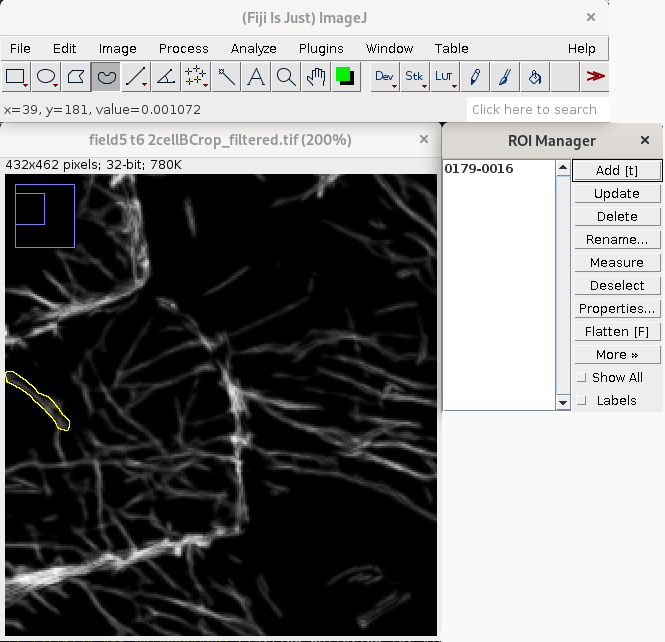
\includegraphics[scale=0.4]{imagenes/IndivManualFijiROI.png}
    \caption[Ejemplo de un filamento individualizado manualmente]{Ejemplo del procedimiento para individualizar manualmente un filamento realizado por un experto en Fiji. Fuente: Elaboraci\'on Propia.}
    \label{fig:roiExample}
\end{figure}

Una vez generadas todas las ROIs que indican los filamentos individualizados por un experto, se genera una segmentaci\'on binaria de la imagen de filamentos. As\'i, los p\'ixeles fuera de las ROIs se clasifican como parte del {\it background} o de segundo plano, con lo que no son consideradas en an\'alisis futuros. Esta imagen resultante es la que puede ser utilizada para extraer un grafo mediante el procedimiento descrito en la secci\'on \ref{subsec:infoLossSkel}.

\section{Resultados algoritmo propuesto en Im\'agenes Sint\'eticas}

La Tabla \ref{tab:Synth-QuantitativeIFS-Fig7DetailedResults1} indica el detalle de las 5 iteraciones utilizadas para promediar el resultado del algoritmo propuesto para las Figura \ref{fig:synth-QFS-7} con la configuraci\'on Modo 2. Por su parte, la Tabla  \ref{tab:Synth-Define-1b-DetailedResults1} muestra los resultados de la individualizaci\'on de filamentos del algoritmo propuesto para la Figura \ref{fig:synth-Define-1b}, con la configuraci\'on definida como Modo 3. Informaci\'on detallada de otros resultados puede encontrarse en el repositorio git del algoritmo propuesto.

\begin{table}[h]
    \centering
    \begin{tabular}{|c|c|c|c|c|c|c|c|c|c|c|c|c|}
    \hline
        Semilla & VI & TP & FP &TN &FN & R	& J & P & R &F1 & C/P & C/GT \\ \hline 
        0    & 0.81 & 9 & 5 & 67 & 10 & 0.83 & 0.37 & 0.64 & 0.47 & 0.54 & 4/6 & 4/6\\
        10 & 0.81 & 9 & 5 & 67 & 10 & 0.83 & 0.37 & 0.64 & 0.47 & 0.54 & 4/6 & 4/6\\
        1271 & 0.27 & 7 & 1 & 37  & 0  & 0.97 & 0.87 & 0.87 & 1 & 0.93 & 4/5 & 4/6\\
        3389 & 0.81 & 9 & 5 & 67 & 10 & 0.83 & 0.37 & 0.64 & 0.47 & 0.54 & 4/6 & 4/6\\
        6821 & 0.81 & 9 & 5 & 67 & 10 & 0.83 & 0.37 & 0.64 & 0.47 & 0.54 & 4/6 & 4/6\\
        \hline
    \end{tabular}
    \caption[Resultados de 5 iteraciones de algoritmo propuesto para individualizar filamentos en la figura \ref{fig:synth-QFS-7}, con la configuraci\'on Modo 2.]{Resultados de 5 iteraciones de algoritmo propuesto para individualizar filamentos en la figura \ref{fig:synth-QFS-7}, con la configuraci\'on Modo 2. El valor m\'aximo de VI en este caso es de 2.3978, ya que el tama\~no del {\it data set} es de 11 aristas. El n\'umero de filamentos en el {\it ground truth} es 6. Las columnas TP, FN, TN y FN corresponden a {\it True Positive}, {\it  False Positive}, {\it True Negative} y {\it False Negative} respectivamente. Por su parte, R y J son los \'indices Rand y Jaccard, P y R son {\it Precision} y {\it Recall}, C/P indica la cantidad de filamentos correctos respecto a los filamentos propuestos, mientras que C/GT son los filamentos correctos en relaci\'on a los filamentos individualizados por un experto.}
    \label{tab:Synth-QuantitativeIFS-Fig7DetailedResults1}
\end{table}


\begin{table}[h]
    \centering
    \begin{tabular}{|c|c|c|c|c|c|c|c|c|c|c|c|c|}
    \hline
        Semilla & VI & TP & FP &TN &FN & R	& J & P & R &F1 & C/P & C/GT \\ \hline 
        0  & 2.14 & 28 & 53 & 263 & 62 & 0.71 & 0.19 & 0.34 & 0.31 & 0.32 & 3/9 & 3/6\\
        10 & 2.09 & 20 & 37 & 261 & 60 & 0.74 & 0.17 & 0.35 & 0.25 & 0.29 & 3/9 & 3/6\\
        1271 & 2.84 & 29 & 63 & 373 & 96 & 0.71 & 0.15& 0.31 & 0.232 & 0.26 & 3/10 & 3/6\\
        3389 & 2.14 & 28 & 53 & 263 & 62 & 0.71 & 0.19 & 0.34 & 0.31 & 0.32 & 3/9 & 3/6\\
        6821 & 1.91 & 19 & 35 & 223 & 48 & 0.74 & 0.18 & 0.35 & 0.28 & 0.31 & 3/9 & 3/6\\
        \hline
    \end{tabular}
    \caption[Resultados de 5 iteraciones de algoritmo propuesto para individualizar filamentos en la figura \ref{fig:synth-Define-1b}, con la configuraci\'on Modo 3.]{Resultados de 5 iteraciones de algoritmo propuesto para individualizar filamentos en la figura \ref{fig:synth-Define-1b}, con la configuraci\'on Modo 3. El valor m\'aximo de VI en este caso es de 2.8332, ya que el tama\~no del {\it data set} es de 17 aristas. El n\'umero de filamentos en el {\it ground truth} es 5. Las columnas TP, FN, TN y FN corresponden a {\it True Positive}, {\it  False Positive}, {\it True Negative} y {\it False Negative} respectivamente. Por su parte, R y J son los \'indices Rand y Jaccard, P y R son {\it Precision} y {\it Recall}, C/P indica la cantidad de filamentos correctos respecto a los filamentos propuestos, mientras que C/GT son los filamentos correctos en relaci\'on a los filamentos individualizados por un experto.}
    \label{tab:Synth-Define-1b-DetailedResults1}
\end{table}

% \section{Resultados Algoritmo algoritmo propuesto en Im\'agenes Reales}

% Las tablas \ref{tab:SpinningMarchantiaDetailedResults1},  \ref{tab:field3t0filteredDetailedResults1} y \ref{tab:field3t0filtered2DetailedResults1} indican el detalle de las 5 iteraciones utilizadas para promediar el resultado del algoritmo algoritmo propuesto en sus respectivos casos. Informaci\'on detallada de otros resultados puede encontrarse en el repositorio del algoritmo algoritmo propuesto.

% \begin{table}[h]
%     \centering
%     \begin{tabular}{|c|c|c|c|c|c|c|c|c|c|c|}
%     \hline
%         Semilla & VI & TP & FP &TN &FN & Rand	& Jaccard &	Precision &	Recall &	F1 \\ \hline 
%         0    & 1.9079 & 43 & 54 & 853 & 85 & 0.8657 & 0.2362 & 0.4432 & 0.3359 & 0.3822 \\
%         10   & 1.7392 & 43 & 51 & 818 & 78 & 0.8696 & 0.25 & 0.4574 & 0.3553 & 0.4 \\
%         1271 & 2.0292 & 44 & 62 & 886 & 89 & 0.8603 & 0.2256 & 0.4150 & 0.3308 & 0.3682 \\
%         3389 & 1.8376 & 43 & 54 & 815 & 78 & 0.8666 & 0.2457 & 0.4432 & 0.3553 & 0.3944 \\
%         6821 & 1.8376 & 43 & 54 & 815 & 78 & 0.8666 & 0.2457 & 0.4432 & 0.3553 & 0.3944 \\
%         \hline
%     \end{tabular}
%     \caption{Resultados de 5 iteraciones de algoritmo propuesto para individualizar filamentos en la figura \ref{fig:SpinningMarchantia}. El valor m\'aximo de VI en este caso es de 3.496508, ya que el tama\~no del {\it data set} es de 29 aristas. El n\'umero de filamentos en el {\it ground truth} es 12.}
%     \label{tab:SpinningMarchantiaDetailedResults1}
% \end{table}
% \addtocounter{table}{-1}
% \begin{table}[h]
%     \centering
%     \begin{tabular}{|c|c|c|c|c|c|c|}
%     \hline
%          & \multirow{4}{2cm}{\centering \% Cobertura de Aristas} & \multirow{4}{2cm}{Filamentos Propuestos} & \multirow{4}{2cm}{Filamentos Correctos} & \multirow{4}{2.5cm}{\% Correctos vs Propuestos} & \multirow{4}{2.5cm}{\centering \% Correctos vs {\it Ground Truth}} & \multirow{4}{1.2cm}{\centering Tiempo [seg]} \\
%          &  &  &  & & &  \\
%         Semilla &  &  &  & & &  \\
%         &  &  &  & & &  \\ \hline 
%         0 & 1 & 13 & 8 & 61.5384 & 66.6667 & 0.7281  \\
%         10 & 1 & 13 & 7 & 53.8461 & 58.3333 & 0.7334\\
%         1271 & 1 & 12 & 7 & 58.3333 & 58.3333 & 0.6870\\
%         3389 & 1 & 12 & 7 & 58.3333 & 58.3333 & 0.6677\\
%         6821 & 1 & 12 & 7 & 58.3333 & 58.3333 & 0.6558\\
%         \hline
%     \end{tabular}
%     \caption{Resultados ({\it Continuaci\'on}) de 5 iteraciones de algoritmo propuesto para individualizar filamentos en la figura \ref{fig:SpinningMarchantia}. El n\'umero de filamentos en el {\it ground truth} es 12.}
% \end{table}


% \begin{table}[h]
%     \centering
%     \begin{tabular}{|c|c|c|c|c|c|c|c|c|c|c|}
%     \hline
%         Semilla & VI & TP & FP &TN &FN & Rand	& Jaccard &	Precision &	Recall &	F1 \\ \hline 
%         0    & 2.0759 & 83  & 82  & 1624 & 164 & 0.8740  & 0.2522  & 0.5030  & 0.3360 & 0.4029 \\
%         10   & 1.8889  & 91  & 81  & 1524 & 134 & 0.8825 & 0.2973 & 0.5290  & 0.4044 & 0.4584 \\
%         1271 & 2.8895 & 107 & 113 & 2430 & 276 & 0.8670 & 0.2157 & 0.4863 & 0.2793 & 0.3548\\
%         3389 & 2.1723 & 108 & 87  & 2022 & 258 & 0.8571 & 0.2332 & 0.5268 & 0.2950 & 0.3782\\
%         6821 & 2.3675 & 91  & 84  & 1873 & 163 & 0.8882 & 0.2692 & 0.52     & 0.3582 & 0.4242\\
%         \hline
%     \end{tabular}
%     \caption{Resultados de 5 iteraciones de algoritmo propuesto para individualizar filamentos en la figura \ref{fig:field3t0filtered1}. El valor m\'aximo de VI en este caso es de 3.7612, ya que el tama\~no del {\it data set} es de 29 aristas. El n\'umero de filamentos en el {\it ground truth} es 12.}
%     \label{tab:field3t0filteredDetailedResults1}
% \end{table}
% \addtocounter{table}{-1}
% \begin{table}[h]
%     \centering
%     \begin{tabular}{|c|c|c|c|c|c|c|}
%     \hline
%          & \multirow{4}{2cm}{\centering \% Cobertura de Aristas} & \multirow{4}{2cm}{Filamentos Propuestos} & \multirow{4}{2cm}{Filamentos Correctos} & \multirow{4}{2.5cm}{\% Correctos vs Propuestos} & \multirow{4}{2.5cm}{\centering \% Correctos vs {\it Ground Truth}} & \multirow{4}{1.2cm}{\centering Tiempo [seg]} \\
%          &  &  &  & & &  \\
%         Semilla &  &  &  & & &  \\
%         &  &  &  & & &  \\ \hline 
%         0 & 1 & 15 & 7 & 46.6666 & 58.3333 & 0.9919  \\
%         10 & 1 & 14 & 8 & 57.1428 & 66.6667 & 1.0342\\
%         1271 & 1 & 16 & 8 & 50  & 66.6667 & 0.9953\\
%         3389 & 1 & 15 & 8 & 53.3333 & 66.6667 & 0.9797\\
%         6821 & 1 & 15 & 8 & 53.3333 & 66.6667 & 0.8456\\
%         \hline
%     \end{tabular}
%     \caption{Resultados ({\it Continuaci\'on}) de 5 iteraciones de algoritmo propuesto para individualizar filamentos en la figura \ref{fig:field3t0filtered1}. El n\'umero de filamentos en el {\it ground truth} es 12.}
% \end{table}

% \begin{table}[h]
%     \centering
%     \begin{tabular}{|c|c|c|c|c|c|c|c|c|c|c|}
%     \hline
%         Semilla & VI & TP & FP &TN &FN & Rand	& Jaccard &	Precision &	Recall &	F1 \\ \hline 
%         0    & 0.428571 & 2 & 1 & 23 & 2 & 0.892857 & 0.4 & 0.666667 & 0.5 & 0.5714 \\
%         10   & 0.428571 & 2 & 1 & 23 & 2 & 0.892857 & 0.4 & 0.666667 & 0.5 & 0.5714 \\
%         1271 & 0.428571 & 2 & 1 & 23 & 2 & 0.892857 & 0.4 & 0.666667 & 0.5 & 0.5714 \\
%         3389 & 0.428571 & 2 & 1 & 23 & 2 & 0.892857 & 0.4 & 0.666667 & 0.5 & 0.5714 \\
%         6821 & 0.428571 & 2 & 1 & 23 & 2 & 0.892857 & 0.4 & 0.666667 & 0.5 & 0.5714 \\
%         \hline
%     \end{tabular}
%     \caption{Resultados de 5 iteraciones de algoritmo propuesto para individualizar filamentos en la figura \ref{fig:field3t0filtered2}. El valor m\'aximo de VI en este caso es de 1.94591, ya que el tama\~no del {\it data set} es de 29 aristas. El n\'umero de filamentos en el {\it ground truth} es 5.}
%     \label{tab:field3t0filtered2DetailedResults1}
% \end{table}
% \addtocounter{table}{-1}
% \begin{table}[h]
%     \centering
%     \begin{tabular}{|c|c|c|c|c|c|c|}
%     \hline
%          & \multirow{4}{2cm}{\centering \% Cobertura de Aristas} & \multirow{4}{2cm}{Filamentos Propuestos} & \multirow{4}{2cm}{Filamentos Correctos} & \multirow{4}{2.5cm}{\% Correctos vs Propuestos} & \multirow{4}{2.5cm}{\centering \% Correctos vs {\it Ground Truth}} & \multirow{4}{1.2cm}{\centering Tiempo [seg]} \\
%          &  &  &  & & &  \\
%         Semilla &  &  &  & & &  \\
%         &  &  &  & & &  \\ \hline 
%         0 & 1 & 5 & 4 & 80 & 80 & 0.2872 \\
%         10 & 1 & 5 & 4 & 80 & 80 & 0.2929\\
%         1271 & 1 & 5 & 4 & 80 & 80 & 0.2882\\
%         3389 & 1 & 5 & 4 & 80 & 80 & 0.2806\\
%         6821 & 1 & 5 & 4 & 80 & 80 & 0.3080\\
%         \hline
%     \end{tabular}
%     \caption{Resultados ({\it Continuaci\'on}) de 5 iteraciones de algoritmo propuesto para individualizar filamentos en la figura \ref{fig:field3t0filtered2}. El n\'umero de filamentos en el {\it ground truth} es 5.}
% \end{table}